\item Problem 25.2-4

(a)

\begin{align*}
    & x_f = 0.413 \\
    & \alpha^* = 10 \\
    & P_l = 20 \\
    & P_h = 80 \\
    x_{0M} &= \frac{x_f \left[1 + \left(\alpha^*-1\right)\frac{P_l}{P_h}\left(1-x_f\right)\right]}{\alpha^*\left(1-x_f\right)+x_f} \\
    x_{0M} &= \frac{0.413 \left[1 + \left(10-1\right)\frac{20}{80}\left(1-0.413\right)\right]}{10\left(1-0.413\right)+0.413} \\
    \Aboxed{x_{0M} &= 0.153}
\end{align*}

(b)

\begin{align*}
    & \alpha^* = 5 \\
    x_{0M} &= \frac{0.413 \left[1 + \left(5-1\right)\frac{20}{80}\left(1-0.413\right)\right]}{5\left(1-0.413\right)+0.413} \\
    \Aboxed{x_{0M} &= 0.196}
\end{align*}

(c)

\begin{align*}
    & \alpha^* = 1 \\
    x_{0M} &= \frac{0.413 \left[1 + \left(1-1\right)\frac{20}{80}\left(1-0.413\right)\right]}{1\left(1-0.413\right)+0.413} \\
    \Aboxed{x_{0M} &= 0.413}
\end{align*}

\begin{center}
    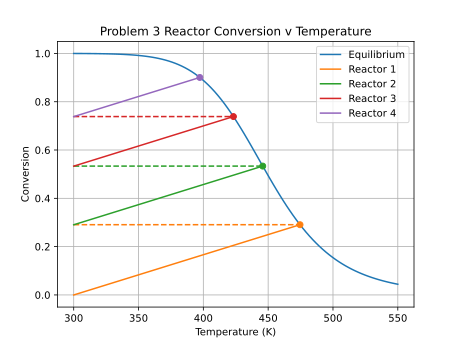
\includegraphics[width=0.8\textwidth]{assets/p3.png}
\end{center}